\chapter{Radzenie sobie z opresją/Przezwyciężanie opresji/Mierzenie się z opresją}
\AddToShipoutPictureBG*{
\includegraphics[width=\paperwidth,height=\paperheight]{TeX_files/3-0.png}}
Artist: Mohammed Fayaz
\newpagek

\begin{figure}[h]
\centering
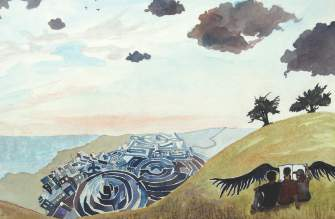
\includegraphics[width=16cm]{TeX_files/3-1.png}
\caption{Artist: Jacks McNamara}
\label{3-1}
\end{figure}

\noindent\textcolor{ProcessBlue}{\textbf{\Large{Jak radzisz sobie z wpływem opresji?}}}\\
\begin{multicols}{2}
\begin{checkboxlist}
\item Przyjaciele
\item Ćwiczenia
\item Zdrowe odżywianie
\item Joga
\item Kreatywna ekspresja
\item Jazda na rowerze
\item Rozciąganie się
\item Walcząc z opresją!
\item Aktywizm!
\item Medytacja
\item Śmiech. Zawsze śmiech
\item Korzystając z portali społecznościowych
\item Śpiew
\item Rysowanie
\item Sztuki walki
\item Natura
\item Icarus [??]
\item Pisanie
\item Bycie częścią społeczności
\item Dowiedz się o niej (opresji) jak najwięcej - [Learn about it]
\item Modląc się o radę - [Pray for guidance]
\item Nie poddając się
\item Zdając sobie sprawę że to nie ze mną jest problem - [Knowing that I am not broken!]
\item Konsultując się z rówieśnikami - [Peer counseling]
\item Wyrabiając sobie swoje własne zdanie - [Owning my opinions]
\item Humor
\item Racjonalizuję ją - [Intellectualizing it]
\item Współczucie
\item Pomaganie innym
\item Czytanie
\item Zabawa ze zwierzęciem
\item Chodzenie na siłownie
\item Praktyki duchowe
\item Terapia
\item Homeopatia
\item Pracuję z własnym ciałem
\item Tulenie/Przytulanie się
\item Rutyna
\item Otwarcie o tym mówiąć
\item Rzeźba
\item Taniec
\item Film
\item Fotografia
\item Solidarność z innymi
\item Sztuka
\item Muzyka
\item Podejmując moje walki
\item Starając się dbać o siebie/uważać na siebie - [Trying to take care of myself]
\item Ucząć się
\item Myśląć
\item Łamiąc stereotypy
\item Robiąc rzeczy które mnie uszczęśliwiają
\item Mówiąc o tym szczerze/otwarcie
\item Pozytywne relacje
\item Przyznając się kiedy nie jest ze mną dobrze - [Admitting when I’m not okay]
\item Przeciwstawiając się jej
\item Edukująć się - [Educating myself]
\item Ograniczająć wystawianie się na opresję - [Limiting exposure to oppressor]
\item Wzmacniając moją miłość własną/samoocenę - [Strengthening my personal love]
\item Rozwijam/wymyślam argumenty - [I developed talking points]
\item Rzecznictwo - [Advocacy]
\item Będąc otwartym na moje wyzwania [Being open about my challenges]
\item Czytając motywujące cytaty, esseje, poematy [Reading empowering statements, essays, and poems]
\item Organizująć się
\item Edukując innych
\item Ucząć się mówić "nie"
\item Nie bać się mówić "prawdy", tak jak jąwidzę [Unafraid to tell the “truth” as I see it]
\item Siła pozytywnego myślenia i działania [Power of Positive Thinking \& Action]
\item Komunikując się z innymi [Communicating to others]
\item Mając wybraną rodzinę [Having a chosen family]
\item Rozpatruję dane zachowanie opresyjne w szerszym kontekście przemocy systemowej dzięki czemu wydaje się ono mniej haniebne [Contextualizing behavior within systemic violence so it is less shameful]
\item Widzę się z moim prawnikiem/wychowawcą/terapeutą [Seeing a counselor.]
\item Pozwalając sobie na płacz/łzy [Allowing ourselves to cry]
\item Czytając o innych ludziach którzy doświadczyli opresji by nie czuć się samotną/ym [Reading about other people who experience oppression in order not to feel alone]
\item Chodząc na wiece [Going to rallies]
\item Pisząć
\item Słuchając wesołej muzyki [Listening to cheerful music]
\item Przypominając sobie że nie każdy będzie nas traktował źle [Reminding ourselves that not everyone will treat us poorly]
\item Przypominając sobie że to sprawcy/oprawcy są winni a nie my [Reminding ourselves that the oppressors are at fault, not us]
\item Pzyjąć uczucie, doświadczyć go w własnym ciele by poźniej się od niego wyzwolić [Acknowledge the feeling, experiencing it in our bodies, and then, after a time, try to let it go]
\item Biorać głębokie oddechy [Take deep breaths]
\item Zmieniając uczucia w działanie: znajdując zdrowe ujście dla wszystkich pasjii i uczuć które muszą być przepracowane [Turning feelings into action: finding a healthy venue for all the passion and emotional work that needs to be done]
\item Ucieczka/Eskapizm w książki lub telewizję jest przyjemna [ Escapism into a book or a TV show is nice]
\item Medytując nad prostotą rozwiazań bez przemocy/opresji - [Meditate on simplicity and non-violent solutions]
\item Zajmując stanowisko - [Taking a stand]
\item Rozwijając dobre relacje z zaufanum lekarzem/personelem medycznym [Developing a good relationship with a trusted healthcare provider]
\item Pozwalając sobie na dzień lub dwa przerwy by się zregenerować [Allow ourselves to take a day or two to recover]
\item Przypominając sobie o tym że życie to nie wyścig - [Remembering that life is not a race]
\item Reiki
\item Detox
\item Ćwiczenia
\item Przebywanie na łonie natury [Being in nature]
\item Opiekując się zwierzętami Caring for animals
\item Wspierająć/pielęgnując ludzi [Nurturing people]
\item Bycie przyjacielem i nauczycielem dal innych
\item Pisanie i czytanie
\item Sztuka
\item Wyrażaniw tego co niewyrażalne
\item Wyżycie się/ Wyładowywanie się
\item Przypomnienie sobie żę kochamy życie - Reminding ourselves that we love life
\item Praktyki duchowe
\item Robienir czegoś więcej niż egzystowanie - [Doing more rather than just existing]
\item Zaangażowanie w troszczenie się o siebie - [Engage in self care]
\item Sięganie po pomoc
\item Głęboki oddech
\item Mówienie do siebie
\item Ćwiczenia
\item Sen
\end{checkboxlist}
\end{multicols}

\newpage
\begin{figure}[h]
\centering
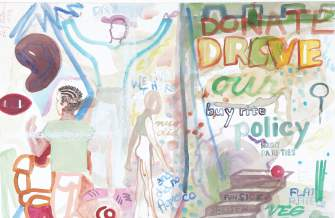
\includegraphics[width=16cm]{TeX_files/3-2.png}
\caption{Artist: Eddy Falconer}
\label{3-2}
\end{figure}

\noindent\textcolor{ProcessBlue}{\textbf{\Large{Jak jeszcze inaczej możesz radzić sobie z wpływem opresji?}}}\\
\noindent\rule{\textwidth}{1pt}\\
\noindent\rule{\textwidth}{1pt}\\
\noindent\rule{\textwidth}{1pt}\\
\noindent\rule{\textwidth}{1pt}\\
\noindent\rule{\textwidth}{1pt}\\
\noindent\rule{\textwidth}{1pt}\\
\noindent\rule{\textwidth}{1pt}\\
\noindent\rule{\textwidth}{1pt}\\
\noindent\rule{\textwidth}{1pt}\\
\noindent\rule{\textwidth}{1pt}\\
\noindent\rule{\textwidth}{1pt}\\
\noindent\rule{\textwidth}{1pt}\\
\noindent\rule{\textwidth}{1pt}\\
\noindent\rule{\textwidth}{1pt}\\\\

\newpage
\noindent\textcolor{ProcessBlue}{\textbf{\Large{Jak radzisz sobie z sytuacjami prowokującymi opresję?}}}\\
\begin{figure}[h]
\centering
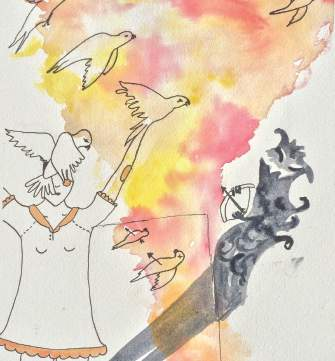
\includegraphics[width=17cm]{TeX_files/3-3.png}
\caption{Artist: Jess Rankine}
\label{3-3}
\end{figure}

\begin{checkboxlist}
\item Staraj się nie dać sprowokować [Try to stay cool]
\item Odetnij się najszybciej jak możesz [Detach as quickly as possible]
\item Słuchjając spokojnej muzyki [Listen to peaceful music]
\item Malująć
\item Doradź osobie która wywołała w tobie uczucie że potrzebujesz chwili przerwy i powiedzmy szklanki wody [Advise the person who triggered the sensation that you need to take a moment and, say, get a glass of water]
\item Zwróć się do innych żerzeli czujesz się przytłoczona/ny [Reach out to others if you feel too overwhelmed]
\item Pozwól by ludzie wiedzieli jak na Ciebie wpływają [Let people know how they are affecting you]
\item Oderwij się albo pójdź na spacer [ Disengage or go for a walk]
\item Rozpoznaj skąd bierze się twoja niepewność [ Recognize where the anxiety is coming from]
\item Pozostań w swojej strefie komfortu z ludźmi których znasz dopóki znajdziesz kogoś komu możesz zaufanego i zwierzysz mu się [Stay in your comfort zone with the people you know until you find someone trusted you can confide in]
\end{checkboxlist}

\noindent\textcolor{ProcessBlue}{\textbf{\Large{Co pomaga Ci radzić sobie w sytuacjach zapalnych [What helps you navigate triggering situations?]}}}
\noindent\textcolor{ProcessBlue}{\textbf{\Large{Jak inni mogą Ci pomóc [How can others help you?]}}}\\
\noindent\rule{\textwidth}{1pt}\\
\noindent\rule{\textwidth}{1pt}\\
\noindent\rule{\textwidth}{1pt}\\
\noindent\rule{\textwidth}{1pt}\\
\noindent\rule{\textwidth}{1pt}\\
\noindent\rule{\textwidth}{1pt}\\
\noindent\rule{\textwidth}{1pt}\\
\noindent\rule{\textwidth}{1pt}\\
\noindent\rule{\textwidth}{1pt}\\
\noindent\rule{\textwidth}{1pt}\\
\noindent\rule{\textwidth}{1pt}\\
\noindent\rule{\textwidth}{1pt}\\
\noindent\rule{\textwidth}{1pt}\\
\noindent\rule{\textwidth}{1pt}\\
\noindent\rule{\textwidth}{1pt}\\
\noindent\rule{\textwidth}{1pt}\\
\noindent\rule{\textwidth}{1pt}\\
\noindent\rule{\textwidth}{1pt}\\\
\newpage

\noindent\textcolor{ProcessBlue}{\textbf{\Large{Jak inni ludzie mogą ci pomóc?}}}
\noindent\textcolor{ProcessBlue}{\textbf{\Large{Jak możemy sobie pomóc na wzajem??}}}\\
\begin{multicols}{2}
\begin{checkboxlist}
\item Nie mów mi: "Otrząśnij się z tego" albo "Wszystko będzie dobrze"
\item Zrób mi herbatę
\item Przynieś mi kwiaty
\item Nie ignoruj mnie
\item Pokaż mi że mnie kochasz
\item Normalize my feelings
\item Przyłąćz się do mnie w działaniu
\item Wesprzyj mnie [Validate me]
\item Wierz
\item Nazwij opresję [Name the oppression]
\item Nawiąż kontakt z innymi którzy mają podobne doświadczenia [Make connections with others who have similar experiences]
\item Validate my experience
\item Normalize
\item Listen to me
\item Say it is not okay
\item Don’t try to fix me
\item Help me up to a better plane of existence
\item Be present
\item Run me a bath
\item Hear and acknowledge the experience
\item Getting me comfy clothes to change into
\item Distract me
\item Tell me a joke or share funny stories
\item Watch a movie with me
\item Talk to me about superficial topics, like celebrities or popular culture
\item Don’t discourage my dreams
\item Believe I am capable of anything despite my struggles and obstacles
\item Educate yourself
\item Help me focus on the things I like
\item Acknowledge that you are capable of racist acts without being racist
\item Appreciate my voice
\item Don’t tell me how I feel
\item Be an ear, even if you don’t agree with me
\item Speak about positive things
\item Engage in intellectual debate
\item Invite me to get together
\item Don’t shoot down my ideas
\item Come visit
\item Treat me like an adult
\item Bring over a treat
\item Tell me that you love me regardless of what happens to me
\item Remembering that it takes me time to heal
\item Stay with me
\item Don’t pressure me
\item Give me space
\item Accept my feelings
\item Be aware
\item Don’t give unsolicited advice
\item Miej cierpliwość/Bądź cierpliwy
\item Przypomnij mi o rzeczach które pomogły mi w przeszłości
\item Bądź wyrozumiały
\item Okaż współczucie
\item Ni mów ,"Dobrze wiem jak się czujesz" - [Don’t say, “I know exactly how you feel”]
\item Przypomnij mi o moich umiejętnościach - [Remind me of my skills]
\item Przytul mnie
\item Pomósz mi użyć moich umiejętności - [Help me use some my skills]
\item Wierz w to co mówię
\item Bądź przy mnie
\item Trzymaj mnie za rękę
\item Nie porzucaj mnie
\item Zaoferuj telefon do mojego terapeuty w moim imieniu - [Offer to call my therapist for me]
\item Pomóż mi redukując napięcie
\item Zaproponuj zajęcie się sprawami - [Offer to run errands]
\end{checkboxlist}
\end{multicols}
\noindent\textcolor{ProcessBlue}{\textbf{\Large{In what other ways can people help you?}}}
\noindent\textcolor{ProcessBlue}{\textbf{\Large{What is helpful? What isn’t?}}}\\
\noindent\rule{\textwidth}{1pt}\\
\noindent\rule{\textwidth}{1pt}\\
\noindent\rule{\textwidth}{1pt}\\
\noindent\rule{\textwidth}{1pt}\\
\noindent\rule{\textwidth}{1pt}\\
\noindent\rule{\textwidth}{1pt}\\
\noindent\rule{\textwidth}{1pt}\\
\noindent\rule{\textwidth}{1pt}\\
\noindent\rule{\textwidth}{1pt}\\
\noindent\rule{\textwidth}{1pt}\\
\noindent\rule{\textwidth}{1pt}\\\\
\newpage
\noindent\rule{\textwidth}{1pt}\\
\noindent\rule{\textwidth}{1pt}\\
\noindent\rule{\textwidth}{1pt}\\
\noindent\rule{\textwidth}{1pt}\\
\noindent\rule{\textwidth}{1pt}\\
\noindent\rule{\textwidth}{1pt}\\
\noindent\rule{\textwidth}{1pt}\\
\noindent\rule{\textwidth}{1pt}\\
\noindent\rule{\textwidth}{1pt}\\
\noindent\rule{\textwidth}{1pt}\\
\noindent\rule{\textwidth}{1pt}\\
\noindent\rule{\textwidth}{1pt}\\
\noindent\rule{\textwidth}{1pt}\\
\noindent\rule{\textwidth}{1pt}\\
\noindent\rule{\textwidth}{1pt}\\
\noindent\rule{\textwidth}{1pt}\\
\noindent\rule{\textwidth}{1pt}\\
\noindent\rule{\textwidth}{1pt}\\
\noindent\rule{\textwidth}{1pt}\\
\noindent\rule{\textwidth}{1pt}\\
\noindent\rule{\textwidth}{1pt}\\
\noindent\rule{\textwidth}{1pt}\\
\noindent\rule{\textwidth}{1pt}\\
\noindent\rule{\textwidth}{1pt}\\
\noindent\rule{\textwidth}{1pt}\\
\noindent\rule{\textwidth}{1pt}\\\
